%%____________________________________________________________________ 
%% File: Introduction.tex
%%____________________________________________________________________ 
%%  
%% Author: Shaun ASHBY <Shaun.Ashby@cern.ch>
%% Update: 2005-11-02 17:04:04+0100
%% Revision: $Id: Introduction.tex,v 1.1 2005/11/02 16:24:18 sashby Exp $ 
%%
%% Copyright: 2005 (C) Shaun ASHBY
%%
%%--------------------------------------------------------------------
\chapter{Introduction}\label{ch:intro}
\index{Introduction}
\scram\ has been developed to enable large, geographically dispersed
and autonomous groups to work together on software development
projects. The groups, primarily based in universities and academic
institutions, independently manage their own resources. As such it can
be extremely difficult or even impossible to impose software process,
adequate documentation levels and heavy resource requirements - such
as dedicating entire machines to a single software development
project.

\section{What is SCRAM?}\index{SCRAM!What is SCRAM?}

\scram\ is a configuration management tool, a distribution system, a
build system and resource manager, with local resources and
applications managed in a transparent way. In addition it provides a
common development environment. These features are described more
fully below.

\subsection{Configuration Management}\label{sec:cm}
\index{SCRAM!configuration management}
The main task of \scram\ is to ensure that all developers are working
with the same consistent set of external products, libraries,
environments and source codes. Configuration management methods ensure
that this is possible.
\begin{description}     
\item [\textsc{external products configuration}]\mbox{}\\
  A requirement of any \scram\ managed project is an explicit
  statement, in the form of a special-purpose document, of all
  underlying products and versions of external libraries and other
  software products used. Each product must have a description
  document to inform \scram\ how it is to be used, to supply dependency
  information, set environmental variables, and give default system
  locations.  Such description documents can be maintained
  independently of \scram\ and imported into the project by
  \scram's built-in URL downloading mechanism.
\item[\textsc{common configurations}]\mbox{}\\
  It is often the case that many projects need to share the same
  configuration in order that they can be inter-operable (\eg two
  applications using the same database).  \scram\ thus provides a
  mechanism for importing independently maintained configuration
  documents automatically.
\item[\textsc{source code control}]\mbox{}\\
  \scram\ itself is not a code repository.  Any project must have
  access to one or more such repositories from which it can checkout
  the appropriate code into the appropriate place in the project
  structure. Currently, CVS is used for all source code management.
  Both source code and project configuration files are tagged with a
  CVS symbolic tag when ready for release.
\item[\textsc{environment control}]\mbox{}\\
  The build and runtime environments are constructed automatically
  from the description documents of the required external products and
  the project-specific environment.
\end{description}


\subsection{The Distribution System}\label{sec:dist}
\index{SCRAM!distribution system}
\index{bootstrapping}
\scram\ projects can be `bootstrapped' from a single description
document in which the structure and download information of other
required project documents and components is declared.

\ni From this document \scram\ can construct a copy of a project release.
Connected to a properly configured web browser such as Netscape makes
automatic project installation possible. At present, \scram\ is unable
to automatically install external components although the user can be
directed to the correct documentation to enable him/her to do this.
Binary distribution is not supported as building a distribution is
seen as a check that all the components of the system have been
installed properly. Other tools, compatible with \scram\, are available
to produce binary distributions from project releases.

\subsection{A System Resource/Application Interface}\label{sec:resource}
\index{SCRAM!resource manager}
\index{SCRAM!application interface}
Often, machines are not installed with the various products in the
same directories, their locations decided upon by system
administrators or system constraints (sizes of filesystems, for
example).  Install locations can also vary from platform to platform.
\scram\ matches up the request for a product in a project configuration
to the system it is installing the project on.  Automated means are
used to achieve this but the user will be prompted if a product cannot
be found. The user also can have full interactive control of these
setup stages if preferred.

\ni A database of system information is maintained by \scram\ for
future reference in each project area.

\subsection{A Build System}\label{sec:bs}
\index{SCRAM!build system}
The build system can be used to build shared or archive libraries, 
plug-in modules, binaries or additional libraries (for a test suite,
for example).  The configuration documents within the project area
describe the actions to be taken during the build process. These
actions can be global, or specific to parts of the source directory
tree structure.  (\eg everything in a directory \texttt{libsrc} could
be automatically compiled into a library or every binary in a
directory called \texttt{test} could be automatically linked with a
test utilities library).
\index{available library classes}
\ni Classes of build objects can be defined: for example, a library class
can have types such as {\em debug}, {\em archive}, {\em shared}, {\em
  shared debug}, \etc Default types can be assigned to a
class/directory structure but can be easily overriden.% with options
%from the command line.  
The environment can be easily tuned for
special cases by simply modifying the templates defining the general
rules.  The dependencies are specified in an abstract manner. Extra 
external products to be included during linking can be referred to 
by name with \scram\ taking care of the system specifics.
\index{module interfaces}
\ni Module interfaces can be defined for large software modules to define
dependencies \etc Other modules can then simply load the interface to
use the module.

\subsection{A Development Environment}\label{sec:de}
\index{SCRAM!development environment}
Once a copy of a project is installed and built on a particular
platform it can be made publicly available (\ie {\em released}) for developers
by adding it to \scram's list of projects (the project database).

\ni Upon selecting an item from this list, a new development area is
created in which the developer can work independently of everyone
else. The development area will have the same configuration and
environment as the base release. It will also automatically use
libraries and headers from the base release if not rebuilt in the
local development area.

\subsection{Project Isolation}
\index{SCRAM!project isolation}
\scram\ ensures that an installed release is independent of any other.
This allows developers to easily switch between projects/versions they
might be working on even though they may have very different and
conflicting environment requirements.
%%
\index{SCRAM!overview}
\begin{latexonly}
  \begin{figure}[ht]
    \begin{center}        
      \leavevmode 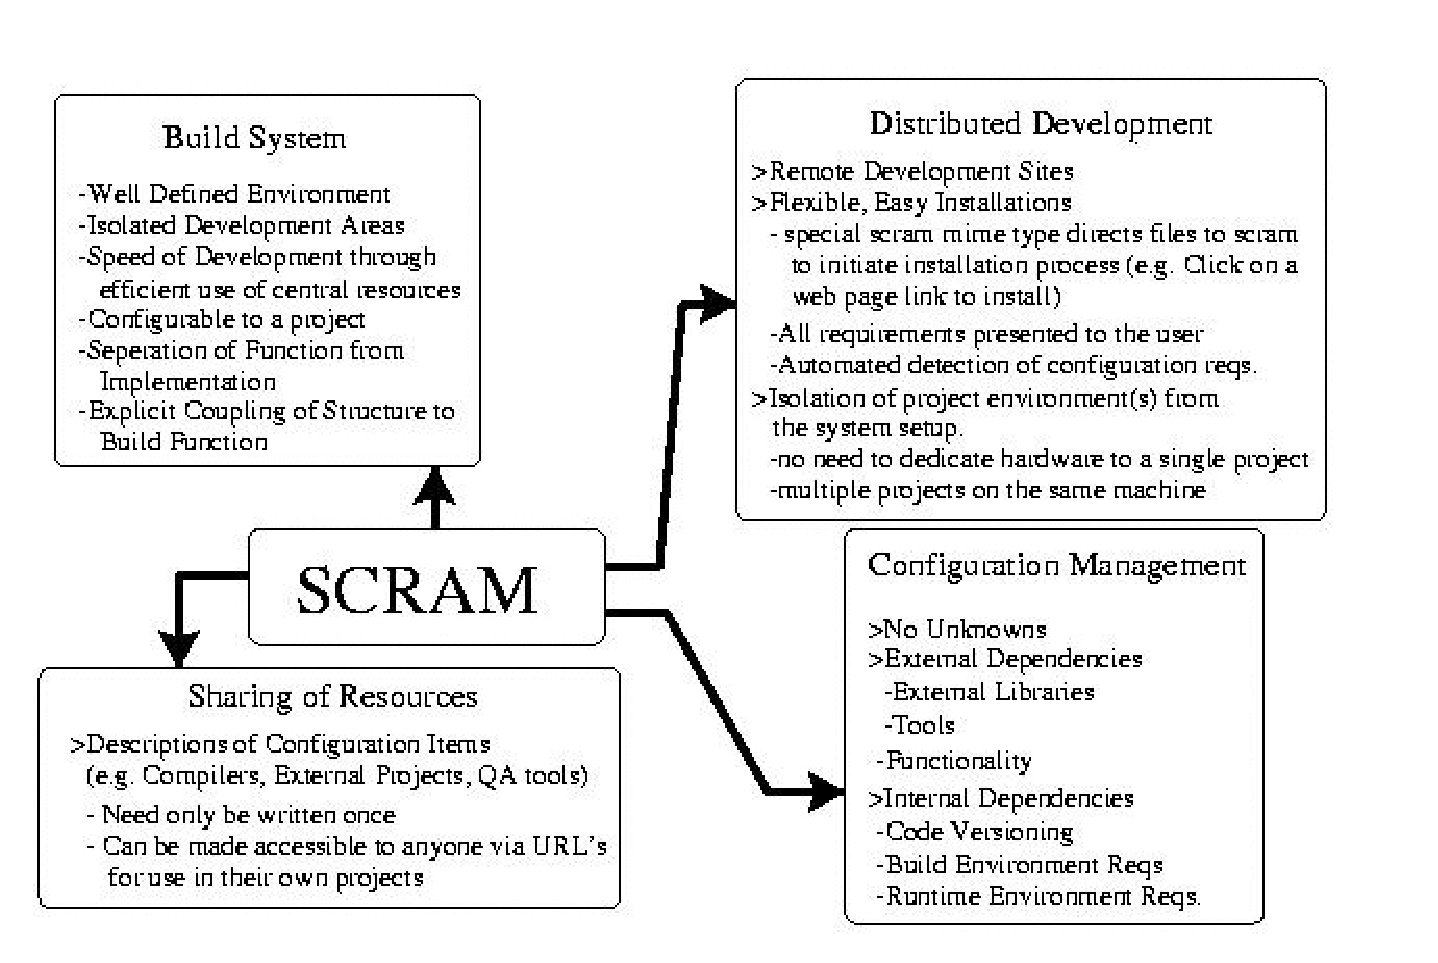
\epsfig{file=images/scram.eps, width=\linewidth}
      \caption[A SCRAM overview.] 
      {A SCRAM overview.}
      \label{f:SCRAM}
    \end{center}
  \end{figure}
\end{latexonly}

\ni In summary, \scram\ can provide
\begin{itemize}
\item project installation with a click on a web page;
\item control of the build environment, including dependency tracking;
\item fully configurable build operations, including default operations;
\item abstraction of logical build elements from the implementation details;
\item re-use of configuration management elements between projects.
\end{itemize}


\section{The Structure of This Guide}

This document can be broken down as follows: firstly,
Chapter~\ref{ch:install} gives some details on how to obtain \scram\
and instructions on how to create a local installation.
Chapter~\ref{ch:creatingprojects} contains all information necessary for
administrators (or users wanting to use \scram\ privately) to
create new projects using \scram\ as the management tool, and to
maintain them. The various types of project configuration files, and
the purposes of each (with use cases), are also described.
Chapter~\ref{ch:examples} serves as a resource for developers who
use \scram\ in their environment, providing some examples and tips covering topics
like changing tool configurations or adding new external tools in a
private area.

\ni Finally there is a summary page containing help for usage for all of
the currently supported \scram\ commands (p~\pageref{ch:quickhelpguide}).

\newpage % Start on a fresh page

%%% Local Variables:
%%% mode: latex
%%% TeX-master: "SCRAM-manual"
%%% End:

%%____________________________________________________________________ 
%% End of Introduction.tex
%%____________________________________________________________________ 
%%  
